% !TEX program = xelatex
\documentclass[runningheads]{llncs}

\usepackage{graphicx}
\usepackage[ruled,vlined]{algorithm2e}
\usepackage{amsfonts}
\usepackage{verbatim}
\usepackage{amsmath}
\usepackage{times} 
\usepackage{tikz}
\usetikzlibrary{automata, positioning, arrows}
\tikzset{
->, % makes the edges directed
>=stealth, % makes the arrow heads bold
node distance=2cm, % specifies the minimum distance between two nodes. Change if necessary.
every state/.style={thick, fill=gray!10}, % sets the properties for each ’state’ node
initial text=$ $, % sets the text that appears on the start arrow
}

\RequirePackage{todonotes}
\newcommand{\znjSide}[1]{\todo[color=orange!10]{\textbf{ZHAN:} #1}}
\newcommand\znj[1]{\textcolor{red}{#1}}
\newcommand{\parseInt}{\textsf{parseInt}}
\newcommand{\paexp}{$\textsf{PA}_{\exp}$}
\newcommand{\Def}{\hat{=}}

\title{A Decision Procedure for String Constraints with String-Integer Conversion and Flat Regular Constraints}
\author{ }
\institute{ } 
\begin{document}
\maketitle{}

\begin{abstract}
    String constraint solving is the core of various testing and verification approaches for scripting languages. 
    Among algorithms for solving string constraints, flattening is a well-known approach that is particularly useful in handling satisfiable instances.
    In the PLDI 2020 paper of Abdulla et al., the authors extended the flattening approach to support the string-integer conversion, which is an important function appearing in almost all scripting languages.
    However, their approach supports only a special flattening pattern and leaves the support of the general flat regular constraints as an open problem.
    In this paper, we fill the gap and propose a complete flattening approach for the string-integer conversion. The approach is built upon a decision procedure for the linear-exponential arithmetic constraints (namely, the extension of Presburger arithmetic with exponential functions) proposed by Point in 1986. While the decision procedure by Point relies on expensive quantifier elimination, we introduce various optimizations and provide an efficient implementation.
%    Besides the theoretical results, we also develop various optimizations and provide an implementation.
    We evaluate the performance of the implementation on the benchmarks that are generated from the string hash functions as well as randomly.
    The experimental results show that our implementation outperforms the state-of-the-art solvers for string-integer conversion constraints as well as linear-exponential constraints, in both precision and efficiency.
\keywords{ String-integer conversion \and Flat regular constraints \and Presburger arithmetic \and Exponential function \and Quantifier elimination.}

\end{abstract}

\iffalse     
    A Decision Procedure for String Constraints with the {\parseInt} Function and Flat Regular Constraints

    {\parseInt} converts strings to integers and is an important function in string manipulating programs. 
    Solving string constraints with {\parseInt} is challenging and undecidable in general. 
    The state-of-the-art string solvers resort to heuristics to solve such constraints. 
    In this work, we propose a decision procedure for a class of string constraints which 
    are boolean combinations of word equations, flat regular constraints, and {\parseInt} function. 
    The decision procedure is obtained by reducing the satisfiability problem to that of
    an extension of Presburger arithmetic with exponential functions, which is decidable. 
    We implement the decision procedure and carry out experiments to evaluate the performance. 
    The experimental results show the improvement against the state-of-the-art string solvers 
    in both precision and performance. To the best of our knowledge, this work represents the 
    first decision procedure for a class of string constraints with {\parseInt} function.
\fi 



\section{Introduction}

solve string constraint is hard

strategy: do unsat and sat separately

strategy: using different procedure to (dis)prove validaity

for disprove validatity, there are two approches, first is bound string length

cannot handle $x.y \neq z  \wedge |x| > 2000$

more recent approach is flattening

it is known that word equaltion + flat regular constraints + len constraints
is decidable

it was unknown that whether word equations + flat regular constraints + len constraints + parseInt is decidable



\section{Preliminaries} \label{sec:pre}

In this section, we introduce some basic concepts and theories that will be used later. 
\subsection{Basic Concepts}

\paragraph{Sets and Strings}
We use $\mathbb{N}$ and $\mathbb{Z}$ to denote the set of natural numbers and integers, respectively. 
$\mathbb{N}^+$ stands for the set of non-zero natural numbers. 
Let $\Sigma$ be a finite alphabet,
a string $w$ over $\Sigma$ is a sequence $a_1....a_n$ of characters from $\Sigma$.
Empty string is denoted by $\epsilon$.
$\Sigma^*$ denotes the set of all finite strings over $\Sigma$,
and $\Sigma_{\epsilon}$ stands for $\Sigma \cup \{\epsilon\}$.
For any string $w_1, w_2\in \Sigma^*$, 
we use $|w_1|$ to denote the length of $w_1$,
and $w_1\cdot w_2$ to denote the concatenation of $w_1$ and $w_2$.
A language $L$ over $\Sigma$ is a subset of $\Sigma^*$.

There are two types of variables in string constraints,
i.e., $X$, a set of string variables ranged over $\Sigma^*$,  
and $Z$,  a set of integer variables ranged over $\mathbb{Z}$.
As usual, an interpretation $I$ is a mapping from the set of variables $X\cup Z$ to the respective domain, 
essentially a pair of two mappings 
$I_X$ and $I_Z$, i.e., $I= (I_X, I_Z)$,  
where $I_X$ is a mapping in $X \mapsto \Sigma^*$ and $I_Z$ is a mapping in $Z \mapsto \mathbb{N}$.

\paragraph{Finite State Automata}
A Finite State Automaton is a tuple 
$\mathcal{A}=\langle Q,\Sigma,\Delta,$ $q_{\textit{init}},$ $q_{\textit{acc}}\rangle$, 
where $Q$ is a finite set of states, 
$\Sigma$ is the given alphabet,
$\Delta\subseteq Q\times \Sigma_\epsilon\times Q$ 
defines the transition relations in $\mathcal{A}$.
$q_{\textit{init}},q_{\textit{acc}}\in Q$ is the initial state and accepting state. 
A sequence $q_0 \langle a_1 \rangle  q_1 ... \langle a_n\rangle q_n$ is called accepting if $q_0 = q_{\textit{init}}$, $q_n = q_{\textit{acc}}$ and $q_{i-1}\langle a_i \rangle q_i \in \Delta$ for $1\le i\le n$.

\paragraph{Presburger Arithmetic} \label{PA}
The Presburger Arithmetic (PA) is a first order theory over signature 
$\Sigma_\mathbb{N}\Def  \{0,1,+,=\}$, where $0,1$ are constants, 
$+$ is a binary function and $=$ is a binary predicate.

PA can be axiomatized by the following axioms \cite{PA} 

\begin{itemize}
    \item $\forall x, \neg (x+1=0)$
    \item $\forall x \forall y. x+1=y+1 \to x=y$
    \item $F(0) \wedge (\forall x. F(x)\to F(x+1)) \to \forall x. F(x)$ 
    \item $\forall x. x+0=x$
    \item $\forall x \forall y. x+(y+1)=(x+y)+1$
\end{itemize}

Given the domain $\mathbb{N}$,
the standard interpretation of PA interprets 
$0,1$ to $0_\mathbb{N},1_\mathbb{N}\in \mathbb{N}$
and $+,=$ to addition and equality over $\mathbb{N}$.
We call a PA formula without quantifiers a quantifier-free PA formula.

PA is a decidable theory, 
and the complexity of decidability is related to 
the number and locations of quantifiers.
Generally, 
the upper bound (on deterministic time and space) 
for deciding a formula of length $n$ is $2^{2^{2^{p n log(n)}}}$,
where $p>1$ is a constant\cite{Oppen69}. 

\paragraph{Parikh Image}
Given an alphabet $\Sigma$ and a string $w\in \Sigma^*$, 
we define the set of Parikh variables 
$\Sigma^\# \Def \{a^\# \mid a\in \Sigma\}$.
The Parikh image of $w$ is a function 
$\mathbb{P}(w): \Sigma^\# \mapsto \mathbb{N}$,
which maps each symbol $a^\#\in \Sigma^\#$ to the number of occurrences
of $a$ in $w$.
For example, let $w\Def aabba$,
then $\mathbb{P}(w)(a^\#)=3,\mathbb{P}(w)(b^\#)=2$.

For a language $L\subseteq \Sigma^*$, 
define the Parikh image of $L$ to be 
$\mathbb{P}(L)\Def \{\mathbb{P}(w) | w\in L\}$.
We say a language $L$ is \emph{Parikh-definable} 
if $\mathbb{P}(L)$ can be characterized by a quantifier-free PA formula over $\Sigma^\#$, 
where $a^\#$ in the formula encodes the number of occurrences of $a$.
It is well known that
any context-free language (therefore regular language) 
is Parikh definable \cite{Parikh66}.

\paragraph{String Terms}
Given a finite alphabet $\Sigma$ and 
a finite set $X$ of string variables over $\Sigma^*$,
we define the set of terms $\textit{Terms}(\Sigma,X)$ 
to be the smallest set satisfying
\begin{itemize}
    \item[1] $\Sigma\cup \{\epsilon\} \cup X \subseteq \textit{Terms}(\Sigma,X)$;
    \item[2] if $t_1,t_2\in \textit{Terms}(\Sigma,X)$, then $t_1 \cdot t_2 \in \textit{Terms}(\Sigma,X)$.
\end{itemize} 

We extend $I_X$ to $\textit{Terms}(\Sigma,X)$ by letting $I_X(\epsilon)=\epsilon$, 
for $a\in \Sigma, I_X(a)=a$,
and $I_X(t_1\cdot t_2)= I_X(t_1)\cdot I_X(t_2)$.

\paragraph{String Constraints} \label{par: string constraints}
Given a constraint $\phi$ and an interpretation $I$,
$I\models \phi$ denotes that $I$ satisfies $\phi$,
and $I$ is called a \emph{model} of $\phi$.
We use $\lVert \phi\rVert$ to denote the set of all models of $\phi$.

We define the following three forms of atomic string constraints:
\begin{itemize}
\item An equality constraint $\phi_e$ is of the form 
$t_1 = t_2$, where $t_1,t_2\in \textit{Terms}(\Sigma,X)$.
We define $\lVert \phi_e \rVert = \{I\mid I(t_1)=I(t_2)\}$.
Inequality constraints can be defined analogously.

\item A regular constraint $\phi_r$ is of the form 
$x\in L(\mathcal{A})$,
where $x\in \mathbb{X}$ and $\mathcal{A}$ is a finite state automaton.
We define $\lVert \phi_r \rVert = \{I\mid I(x)\in L(\mathcal{A})\}$.

\item A length constraint $\phi_l$ is a linear constraint over 
$Z \cup \{|x| \mid x\in X\}$, %the values of $|x|$ for all $x\in X$,
where $|\cdot |$ is the length function.
We define $\lVert \phi_l \rVert = \{I \mid I\models \phi_l \}$.
\end{itemize}

In Section~\ref{sec:string-solving},  
we will introduce a new form of atomic string constraints, i.e., \emph{string-number conversion constraints}.
A string constraint is a Boolean combination of atomic string constraints possibly with quantifications over $X\cup Z$. Other notions are same as in the first-order logic. 

Giving a string constraint $\Psi$,
the problem of string constraints solving is to decide 
whether $\lVert \Psi \rVert$ is empty,
if not, to compute an interpretation $I$ that satisfies $\Psi$.


\subsection{Flat Automata and Flat Languages}

Given a string constraint $\Psi$,
the general problem of deciding whether $\lVert \Psi \rVert$ is empty is undecidable.
However, 
the problem becomes decidable when certain restrictions are imposed.
One of the restriction is by flat automata and flat languages, 
defined below. 

\paragraph{Flat Languages and Automata}
For a fixed alphabet $\Sigma$,
we say a language $L$ over $\Sigma$ to be \emph{$\langle p,q \rangle$-flat} if 
there exist strings $w_1,...,w_q \in \Sigma^*$ such that
$|w_i|\le p$ for all $i:1\le i \le q$ 
and $L = (w_1)^*(w_2)^*...(w_q)^*$. 
We use $\alpha$ to denote $\langle p,q \rangle$, 
and call it the \emph{abstraction parameter} of $L$.
Intuitively,
a flat language with abstraction parameter $\alpha = \langle p,q \rangle$
consists of $q$ loops and the length of each loop body is equal or less than $p$.
For example,
$L = (ab)^*(a)^*(bb)^*$ is a $\langle 2,3 \rangle$-flat language.

Flat automata are a special form of finite state automata that 
recognize flat languages.
Fix the abstraction parameter $\alpha=\langle p,q\rangle$,
a flat automaton consists of $q$ loops,
each loop is a circle of $p$ states.
Formally, 
an $\alpha$-flat automaton contains $p q$ states at most,
and we name the states from $1$ to $p q$,
$1$ is the initial state and $(p q - p + 1)$ is the accepting state.
We use $\cdot$ as a placeholder for some symbol in $\Sigma_\epsilon$,
the transition relations of state $i$ are defined as 
\begin{itemize}
    \item if $i\  \text{mod}\  p = 1$ and $i \neq pq-p+1$, then 
    $(i,\epsilon,i+p)\in \Delta$,
    $(i, \cdot ,i+1) \in \Delta$;
    \item if $i\  \text{mod}\  p = 0$, then 
    $(i,\cdot , i-p+1) \in \Delta$;
    \item otherwise, $(i,\cdot, i+1) \in \Delta$.
\end{itemize}

A $\langle 2,3 \rangle$-flat automaton 
that recognizes $L\Def  (ab)^*(a)^*(bb)^*$ is shown in 
figure (\ref{fig: FA}).


\begin{figure}[ht]
    \centering 
    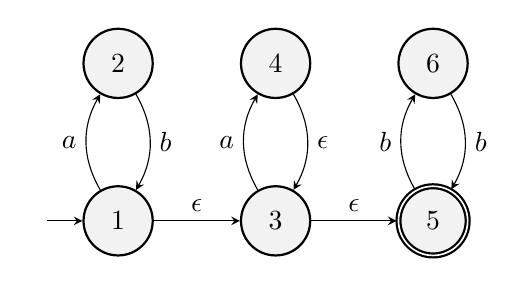
\begin{tikzpicture}
        \node[state,           ] (4) {$4$};
        \node[state, left  of=4] (2) {$2$};
        \node[state, right of=4] (6) {$6$};
        \node[state, initial, below of=2] (1) {$1$};
        \node[state, below of=4] (3) {$3$};
        \node[state, accepting, right of=3] (5) {$5$};
        
        \draw 
        (1) edge[above] node{$\epsilon$} (3)
        (3) edge[above] node{$\epsilon$} (5)
        
        (1) edge[bend left,left] node{$a$} (2)
        (2) edge[bend left,right] node{$b$} (1)
        
        (3) edge[bend left,left] node{$a$} (4)
        (4) edge[bend left,right] node{$\epsilon$} (3)
        
        (5) edge[bend left,left] node{$b$} (6)
        (6) edge[bend left,right] node{$b$} (5);
    \end{tikzpicture}
    \caption{A $\langle 2,3 \rangle$-flat automaton 
that recognizes $L\Def  (ab)^*(a)^*(bb)^*$}
    \label{fig: FA}
\end{figure}

 
\paragraph{Generic Flat Languages and Automata}
Fix $\alpha = \langle p,q \rangle$,
we define the \emph{generic $\alpha$-flat language} is the union of all $\alpha$-flat languages, denoted by $\mathbb{F}(\alpha)$.
Now, we try to define an automaton that recognizes all $\alpha$-flat languages,
i.e., collects all behaviors of $\alpha$-flat automata.

Intuitively, 
the generic automaton is obtained by introducing a new alphabet (
a multi-set with $p q$ copies of the original alphabet) and 
adding more transitions (labels),
the states and the overall framework remain unchanged. 
In details, a generic $\alpha$-flat automaton is still a finite state automaton over
$\Sigma(\alpha)\Def \{a(i)| (a\in \Sigma_\epsilon) \wedge i\in \mathbb{N}:1\le i \le pq\}\cup \{\epsilon\}$.
The states are still named from $1$ to $pq$, 
the initial state is $1$ and the accepting state is $(pq-p+1)$.
The transition relations for state $i$ are defined as 
\begin{itemize}
    \item if $i\  \text{mod}\  p = 1$ and $i\neq pq-p+1$, then 
    $(i,\epsilon,i+p)\in \Delta$
    and $\forall s\in \Sigma_{\epsilon}. (i, s(i) ,i+1) \in \Delta$;
    \item if $i\  \text{mod}\  p = 0$, 
    $\forall s \in \Sigma_{\epsilon}. (i,s(i), i-p+1) \in \Delta$;
    \item otherwise, $\forall s \in \Sigma_{\epsilon}. (i,s(i), i+1) \in \Delta$.
\end{itemize}

For $\Sigma = \{a,b\}$, an example of generic $\langle 2,3 \rangle$-flat automaton is shown in figure (\ref{fig: GFA}).

\begin{figure}[ht]
    \centering 
    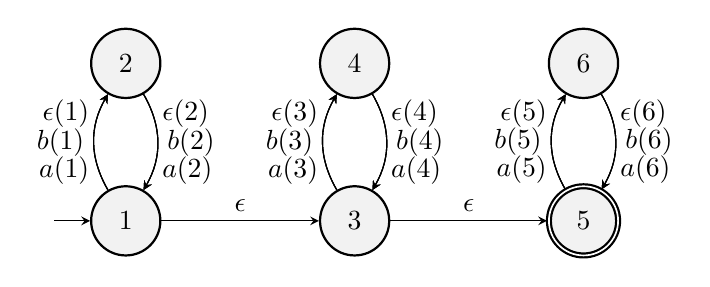
\begin{tikzpicture}
        \node[state,           ] (4) {$4$};
        \node[state, left  = 2cm of 4] (2) {$2$};
        \node[state, right = 2cm of 4] (6) {$6$};
        \node[state, initial, below of=2] (1) {$1$};
        \node[state, below of=4] (3) {$3$};
        \node[state, accepting, below of=6] (5) {$5$};
        
        \draw 
        (1) edge[above] node{$\epsilon$} (3)
        (3) edge[above] node{$\epsilon$} (5)
        
        (1) edge[bend left, pos =0.2 ,left] node{$a(1)$} (2)
        (1) edge[bend left, pos =0.5 ,left] node{$b(1)$} (2)
        (1) edge[bend left, pos =0.8 ,left] node{$\epsilon(1)$} (2)
        
        (2) edge[bend left, pos = 0.2 ,right] node{$\epsilon(2)$} (1)
        (2) edge[bend left, pos = 0.5 ,right] 
        node{$b(2)$} (1)
        (2) edge[bend left, pos = 0.8 ,right] 
        node{$a(2)$} (1)
        
        (3) edge[bend left, pos =0.2 ,left] node{$a(3)$} (4)
        (3) edge[bend left, pos =0.5 ,left] node{$b(3)$} (4)
        (3) edge[bend left, pos =0.8 ,left] node{$\epsilon(3)$} (4)
        
        (4) edge[bend left, pos = 0.2 ,right] node{$\epsilon(4)$} (3)
        (4) edge[bend left, pos = 0.5 ,right] 
        node{$b(4)$} (3)
        (4) edge[bend left, pos = 0.8 ,right] 
        node{$a(4)$} (3)
        
        (5) edge[bend left, pos =0.2 ,left] node{$a(5)$} (6)
        (5) edge[bend left, pos =0.5 ,left] node{$b(5)$} (6)
        (5) edge[bend left, pos =0.8 ,left] node{$\epsilon(5)$} (6)
        
        (6) edge[bend left, pos = 0.2 ,right] node{$\epsilon(6)$} (5)
        (6) edge[bend left, pos = 0.5 ,right] 
        node{$b(6)$} (5)
        (6) edge[bend left, pos = 0.8 ,right] 
        node{$a(6)$} (5);
    \end{tikzpicture}
    \caption{The generic $\langle 2,3 \rangle$-flat automaton}
    \label{fig: GFA}
\end{figure}
 

However,
the resulted automaton may accept languages that are not in $\mathbb{F}(\alpha)$,
because in different passes inside a loop, 
the automaton can choose different symbols between identical pairs. 
To avoid this problem,
we add a so-called purity condition on the accepting language of generic flat automata,
which is equivalent to intersecting the language of a generic flat automaton 
with a language that encodes the purity condition.

We say a string $w\in (\Sigma(\alpha))^*$ is pure if for all $i: 1\le i \le p q$,
and $a,b\in \Sigma$, 
$a\neq b \wedge \#w(a(i))>0$ implies $\#w(b(i))=0$.
Formally, the purity condition is defined by 
\begin{equation} \label{eq:purity}
 \bigwedge_{1\le i\le pq}\bigwedge_{a,b\in \Sigma, a\neq b} ({a(i)}^\#>0)\to ({b(i)}^\#=0)\, . 
\end{equation}

We denote the accepting language of the generic $\alpha$-flat automaton by $\mathbb{G}(\alpha)$.
Note that $\mathbb{G}(\alpha)$ is a language over $\Sigma_\alpha$,
but what we want is a language over $\Sigma$.
So we define a renaming function $R:\Sigma(\alpha)\mapsto \Sigma$ such that for all $a(i) \in \Sigma_\alpha, R(a(i))=a$,
and $R(\epsilon) = \epsilon$.
Define $\mathbb{G}'(\alpha) \, \Def \, \{R(w) \mid w\in \mathbb{G}(\alpha)\}$, 
for simplicity, we write
$\mathbb{G}'(\alpha)=R(\mathbb{G}(\alpha))$.

The important feature of generic flat autamata
is that every word $w\in \mathbb{G}(\alpha)$ is uniquely determined by its Parikh image $\mathbb{P}(w)$.


\subsection{Flattening}

The flattening technique was first introduced 
in \cite{Abdulla 2017}.
Fix an alphabet $\Sigma$ and an abstraction parameter $\alpha$, 
for a given atomic string constraint $\phi$, 
flattening $\phi$ with parameter $\alpha$ 
results in a new string constraint $\phi_\alpha$,
such that 
$R(\lVert \phi_\alpha \rVert) = \lVert \phi \rVert \cap \{I \mid \forall x\in X, I(x)\in \mathbb{G}'(\alpha)\}$,
where $R$ is the renaming function with its domain extended to interpretations in the normal manner.
Intuitively, it restricts $\phi$ to interpret 
string variables over $\mathbb{G}'(\alpha)$.

\cite{Abdulla 2017} discussed the flattening of basic 
string constraints including equality, integer, (regular) grammar and transducer constraints. 
For an atomic string constraint $\phi$,
the flattening $\phi_\alpha$ is still an atomic string constraint 
and is Parikh definable,
so its Parikh image can be expressed by a quantifier free PA formula.
Together with the purity condition,
we obtain an existential quantified PA formula $\rho$.
$\rho$ will be sent to a SMT solver,
if the solver returns an solution $\theta$,
then we can construct an interpretation for $\phi_\alpha$ from $\theta$,
otherwise it means $\phi$ is unsatistiable when 
string variables are interpreted  to $\alpha$-flat languages.

Take a regular constraint $\phi = x\in L(A)$ for example,
the flattening of $\phi$ resutls in a new finite state automaton $A'$ over $\Sigma(\alpha)$,
which encodes running $A$ ``in parallel" 
with the generic $\alpha$-flat automaton.
Let $\rho_1$ be the formula describing the Parikh image of $A'$,
which is a formula over variable sets $\Sigma(\alpha)^\#$.
Let $\rho_2$ be the purity condition \eqref{eq:purity}.
Then we obtain the PA formula $\exists (\Sigma(\alpha))^\#. \rho_1 \wedge \rho_2$.
In order to distinguish between different string variables,
we may replace $a(i)^\# \in \Sigma(\alpha)^\#$ by $(x,a(i))^\#$.

Since the structure of a flat automaton is decided 
by its abstraction parameter $\alpha$, 
a Counter-Example Guided Abstraction 
Refinement (CEGAR) framework is designed, which contains both an under- and an 
over-approximation module, to search the possible values of $\alpha$.
The termination for the overall algorithm is not guaranteed.

\section{Solving String Constraints with \textsf{parseInt} Function}\label{sec:string-solving}

The string-number conversion functions are commonly used functions
in most of programming languages,
for example,
\verb+parseInt()+ in Java and \verb+Int()+ in Python.
The functions usually take two parameters, 
a string over the agreed alphabet $\Sigma$
and an optional parameter denotes the radix.
They parse the string according to the rules indicated by the radix,
and return an integer denoted by the string.

From the view of string constraints,
string-number conversion functions give rise to a new form of string constraints
and are more expressive than length constraints.
So we consider extending string constraints with 
{\parseInt} function. 
As the general problem of string constraints is undecidable,
we still adopt the idea of flattening, 
i.e., variables are restricted to (generic) flat languages.
This problem has been investigated in \cite{POPL20},
which defined a special form of flat restriction (straight-line PFA) and 
proposed a heuristic search method.

In this section, 
we describe the problem of interest first, and then 
present an reduction from the problem of solving flat string constraints with {\parseInt} function
to the decidability problem of Presburger Arithmetic with exponential functions.
Hence, we identify a decidable subset of string constraints, which is the largest one with decidability so far to the best of our knowledge.

\subsection{String-Number Conversion Function}

Commonly, 
{\parseInt} function takes a string representation of a decimal
number and returns an integer.
Since we focus on the decidability,
we define a binary version of {\parseInt},
which takes a binary string and returns a decimal integer number.
For example,
${\parseInt}('111')=7$. 
Clearly,  our decision procedure given in this paper 
can be adapted to string constraints with other string to number conversion function without substantial change. 
Single quotation marks are used to distinguish a symbol like $'1'\in \Sigma$
from a number $1_\mathbb{N}\in \mathbb{N}$ when needed.


\begin{definition} Let $\Sigma_{\textit{num}}=\{'0','1'\}$,
 ${\parseInt}:\Sigma_{\textit{num}}^*\mapsto \mathbb{N}$ is recursively defined by:
    for $w\in \Sigma_{\textit{num}}^*$
    \begin{itemize}
        \item if $|w|=0$, i.e., $w=\epsilon$,  ${\parseInt}(w)=0$;
        \item if $|w|=1, {\parseInt}('w')=w_\mathbb{N}$;
        \item for $|w|\ge 2$ and $w=w_1 \cdot w_2$, 
        where $|w_1|, |w_2| \ge 1$, 
        ${\parseInt}(w) = {\parseInt}(w_1)2^{|w_2|}+{\parseInt}(w_2)$.
    \end{itemize} 
\end{definition}

Now, we introduce a new form of atomic string constraints: 
a {\parseInt} constraint $\phi$ is of the form 
$n \sim {\parseInt}(t)$,
where $n$ is an integer term, $\sim \in \{\le,<,=,>,\ge\}$ and $t\in \textit{Terms}(\Sigma_{\textit{num}},X)$ is a string term.
$\lVert \phi\rVert \Def  \{I \mid I(n)\sim {\parseInt}(I(t))\}$.

In what follows, we only  consider the problem in the case when $t=x$ and $x$ is restricted to (generic) flat languages. 
%If $t$ is not a single variable, 
For the general case $t\in \textit{Terms}(\Sigma_{\textit{num}},X)$, 
it can be reduced to this special case by induction on the structure of $t$. 
%we can reduce the problem by separating $t$ (corresponding to the $|w|>2$ case in definition).

Given an $\alpha$-flat language $L$,
we assume $\alpha=\langle p,q \rangle$ and $L=(w_1)^*...(w_q)^*$,
where $p,q$ and $w_i(1\le i \le q) $ are known.
We further assume that $x = (w_1)^{\beta_1} ... (w_q)^{\beta_q}$,
then we have
\begin{align}
    &{\parseInt}(x) \notag \\
    =&{\parseInt}((w_1)^{\beta_1} ... (w_q)^{\beta_q}) \notag \\
    =&{\parseInt}((w_1)^{\beta_1} ... (w_{q-1})^{\beta_{q-1}})\cdot 2^{\beta_q |w_q|}
    + {\parseInt}((w_q)^{\beta_q}) \label{parse}
\end{align}
(\ref{parse}) is a recursive expression.
So we only need to deal with the basic case ${\parseInt}((w_q)^{\beta_q})$, 
where $w_q \neq \epsilon$
\begin{align}
    {\parseInt}((w_q)^{\beta_q}) &= \sum_{i=0}^{\beta_q-1} {\parseInt}(w_q)\cdot 2^{|w_q|\cdot i}  \notag \\
    &={\parseInt}(w_q)\frac{2^{|w_q|\cdot \beta_q}-1}{2^{|w_q|}-1}
    \label{parseInt-basic}
\end{align}
In (\ref{parseInt-basic}), since $w_q$ and $|w_q|$ are known, 
they can be regarded as constants.
The only unknown variable is $\beta_q$.

Combine (\ref{parse}) and (\ref{parseInt-basic}),
the constraint $n={\parseInt}(x)$ can be expressed by an arithmetic expression with 
$n$ and $(\beta_1,...,\beta_q)$,
inevitably with exponential components.

Take $n={\parseInt}((11)^a(10)^b)$ for example.
\begin{align}
    n=& {\parseInt}((11)^a)\cdot 2^{2b} + {\parseInt}((10)^b) \notag \\
    =& {\parseInt}(11)\cdot \frac{2^{2a}-1}{2^2-1}\cdot 2^{2b} + 
    {\parseInt}(10) \cdot \frac{2^{2b}-1}{2^2-1} \notag 
\end{align}

So we have 
\begin{equation}
    3\cdot n = 3\cdot 2^{2a+2b}-3\cdot 2^{2b}+2\cdot 2^{2b}-2. \notag
\end{equation}

Observe the form of the above equation,
$a,b,n$ are integer variables and either occur in 
an exponential term or a linear term.
This is always the case,
so the problem can be reduced to 
the decidability of PA with exponential function.

When $x$ of {\parseInt} constraints is restricted to the
generic $\alpha$-flat language ($\alpha$ is fixed),
the (\ref{parse}) and (\ref{parseInt-basic}) still hold 
but $w_i(1\le i\le q)$ is known.
However,
by definition,
the generic $\alpha$-flat language is the finite union of all $\alpha$-flat languages,
so we can enumerate all possible values for $w_i$.
In this way,
the problem can still be reduced to the decidability of PA with exponential function (\paexp), i.e.,
\begin{theorem} \label{thm:string-parInt}
If {\paexp} is decidable, then the satisfiability (validity) of string constraints with {\parseInt} in which all string variables 
are ranged over flat strings is decidable. 
\end{theorem}


\subsection{Decidability of \paexp} \label{sec:3.2}

For a first order theory $T$,
we say theory $T$ admits quantifier elimination (QE) if for any formula in $T$, 
there is a quantifier-free formula equivalent to it.
It is well-known that if a theory admits QE, 
then it is a decidable theory.

The formal definition of PA is given in section \ref{PA}.
Here we add the ordering predicate $\le$ into the signature,
which can be defined by $x \le y\, \Def \, \exists z. x+z=y$.
However, the theory PA so far does not admit QE, 
for example, consider the formula $\exists x.x = y + y$. 
We augment the theory with countable unary divisible predicates
$n|x$, where $n\in \mathbb{N}$, 
$n|x$ is true if and only if $x\ \text{mod}\ n=0$ holds.
This structure of PA that admits QE is denoted by $(\mathbb{N},+)$.

We then introduce a theory {\paexp}, denoted by $(\mathbb{N},+,2^x)$, that we work on.
\begin{definition}
    Let $\mathcal{L}=\{0,1,+,\le,n \, |x(n\in \mathbb{N}),2^x,l_2(x)\}$, 
     $(\mathbb{N},+,2^x)$ be a $\mathcal{L}$-theory that has domain $\mathbb{N}$, where 
    \begin{itemize}
        \item  $2^x$ is interpreted to the exponential function of $2$ over $\mathbb{N}$; 
        \item interpretations of $0,1,+,\le,=$ are consistent with PA;
        \item for $n\ge 1$,$n|x$ holds iff $\exists y.x=ny$;
        \item $2^0=1$, for $n \ge 1, 2^n = 2^{n-1}+2^{n-1}$;
        We further assume that if $m,n\in \mathbb{N}, m\le n$, 
        then $2^{m-n} = 1$
        \item $l_2(0)=0$; for $n \ge 1,l_2(n) = y$ iff $2^y \le n < 2^{y+1}$;  $l_2(m-n) = 0$
        if $m,n\in \mathbb{N}$ and $m\le n$. 
    \end{itemize}
\end{definition}

$\lambda_2(x) = 2^{l_2(x)}$ can be defined by $l_2(x)$,
intuitively, $\lambda_2(x)$ means the maximal power of 2 that is not larger than $x$.
Then we have $\lambda_2(x) \le x \le 2\lambda_2(x)-1$,
which will be useful in our proof. 

\begin{definition}
    For a strictly increasing function $f:\mathbb{N}\mapsto \mathbb{N}$, 
    $f$ is said to be compatible with addition 
    if for every $m\in \mathbb{N}^+$,  $f$ modulo $m$ is periodic, 
    and for any term $A(x)=\sum_{1\le i\le n} a_i f(x+b_i)$, 
    where $n \in \mathbb{N}^+, a_i ,b_i \in \mathbb{Z}$,
    one of the following holds:
    \begin{itemize}
        \item $A(x)$ is bounded; 
        \item there exists a constant $\Delta_A\in \mathbb{N}^+$ such that 
        $\forall x. A(x+\Delta_A)\ge f(x)$;
        \item there exists a constant $\Delta_A\in \mathbb{N}^+$ such that 
        $\forall x. -A(x+\Delta_A)\ge f(x)$.
    \end{itemize}
\end{definition}

%\znjSide{\textbf{Solved}. I think you need to explain the meanings of compatibility.}

Semenov proved that for any function $f$ that is compatible with addition, 
theory $(\mathbb{N},+,f)$ admits QE  and thus the theory is complete and decidable \cite{Semenov84}. 
Exponential functions are compatible with addition functions, and therefore {\paexp} is decidable 
by \cite{Semenov84}.
Particularly, in \cite{Point86} Point gave a detailed QE algorithm for $(\mathbb{N},+,2^x)$, where $f(x)=2^x$.
Unfortunately, Point's algorithm is flawed, one problem 
 lies in the discussion to eliminate exponential terms. 
% making the algorithm fail to handle "$a_0<0$" case.
For example, after  eliminating variable $x$ in formula $\exists x. y\le 2^x \wedge x\le 10$,
the expected result should be $y\le 2^{10} =1024$,
but Francoise's algorithm will return a formula equivalent to $y \le 2^6=64$.
% 这里好像还有另一个与Francoise一起的作者

In the next section, within Point's framework, we give a revised algorithm
 to the decision problem of {\paexp} with 
both subtle improvements and crucial corrections, that 
provides a crucial step to the decision procedure of string constraints with {\parseInt} function according to 
Theorem~\ref{thm:string-parInt}. 



\section{Quantifier Elimination Algorithm for $(\mathbb{N},+,2^x)$}
Based on Point's work \cite{Point86}, we present a  revised QE algorithm for the formula of the form $Qx.\theta(x,\bar{y})$, 
where $Q$ is a quantifier and $\theta(x,\bar{y})$ is a quantifier-free formula. 
Since $\forall x. F = \neg \exists x. \neg F$, we further assume the quantifier $Q$ to be the existential quantifier, 
that is, $\exists x.\theta(x,\bar{y})$. 
For eliminating quantifiers in arbitrary formula, 
we apply the algorithm to the innermost quantified formula and repeat this procedure until all quantifiers are eliminated.

We divide the whole QE algorithm into 4 steps.
The first step $\textbf{Normalization}$ can be viewed as a pre-processing step, which substitutes ``complex" terms like $2^{2^x}$, $l_2(3x+y)$ with ``simple" terms by introducing new variables $x_i$. Now we move forward to handle a ``simpler" formula, however, at the cost of more quantified variables.

The other three steps undertake the task to eliminate the introduced variables $x_i$ and the original variable $x$ (will be denoted by $x_0$) one by one. 
The main body of \textbf{QE-with-Order} step is a loop to enumerate all possible orders among quantified variables. 
In each iteration, according the given (decreasing) order (corresponding to a for loop), we invoke \textbf{QE-exp} or 
\textbf{QE-linear} to eliminate these variables one by one. 
%depending on  eliminates the maximal variable in the remaining $\bar{x}$. So it is necessary to specify an ordering for $\bar{x}$ at the beginning, as we will see, this is the main reason for the complexity of this algorithm.
During each iteration of the inner loop (the for loop), 
if the maximal $x_i$ in $\bar{x}$ occurs in an exponential term in an atomic formula, 
we will invoke \textbf{QE-exp} to produce a formula equivalent to the atom where $x_i$ occurs linearly;  
otherwise, if $x_i$ occurs linearly in the formula, \textbf{QE-linear} will be invoked to eliminate all occurrences of $x_i$, 
and this procedure is similar to the classic QE algorithm for PA. 

A more detailed description is given below.

\subsection{Normalization}

In order to show $(\mathbb{N},+,2^x)$ admits QE , 
it is sufficient to show that any 1-existential formula $\exists x.\theta(x,\bar{y})$ indeed does, 
where $\theta(x,\bar{y})$ is a quantifier-free formula. 
However, the form of $\exists x.\theta(x,\bar{y})$ is unknown so it may contain terms difficult to handle such as $2^{3x+y+1}$ or $l_2(x)$.
The \textbf{Normalization} step simplifies these terms by introducing new variables, 
for example, $\exists x.2^{3x+y+1}>10$ is equivalent to
$$\exists x\exists x_1.2^{x_1}>10 \wedge x_1 =3x+y+1\,.$$

Logarithm functions are replaced by exponential functions, take $\exists x.l_2(x)>3$ for example, $l_2(x)$ is replaced by a new variable $x_1$, and we have  
$$\exists x\exists x_1. x_1 > 3 \wedge 2^{x_1}\le x \wedge x\le 2^{x_1+1}-1\,.$$

The \textbf{Normalization} step goes like this, first transform the given formula $\theta(x,\bar{y})$ into the Negation Normal Form (NNF).
Then $\theta(x,\bar{y})$ becomes a Boolean combination (with only $\wedge$ and $\vee$) of literals.

Make substitutions by introducing new variables according to the \textit{while} statements in the pseudo-code.For consistency, we rename the original $x$ to be $x_0$ and assume $n$ new quantified variables are introduced.

After introducing new variables and substitution, 
we obtain a formula where if an exponential term contains a quantified variable $x_i(0\le i\le n)$, the term should be $2^{x_i}$.
We then collect all terms with $x_i(0\le i\le n)$ together, 
it will be of the form $s(\bar{x})\Def \sum_{i=0}^{n} a_i 2^{x_i} + \sum_{i=0}^n b_i x_i$, where $a_i,b_i(0\le i \le n)$ are all constants.
Other terms including constants and terms of $\bar{y}$ are collected,  
denoted by $t(\bar{y})$. 
Since $\bar{y}$ are free variables, 
we will regard $t(\bar{y})$ as a constant.
Inequalities and equalities will all be transformed into $s(\bar{x})\le t(\bar{y})$, for example, $s(\bar{x}) = t(\bar{y})$ will be replaced by $s(\bar{x})\le t(\bar{y})\wedge t(\bar{y})\le s(\bar{x})$.

At the end, the resulted formula $\theta'$ only contains literals of the forms $s(\bar{x})\le t(\bar{y})$, $k|s(\bar{x})+t(\bar{y})$ and $\neg  (k|s(\bar{x})+t(\bar{y}))$.


\begin{algorithm}[t]
    \SetAlgoLined
    \KwIn{1-existential formula $\exists x.\theta(x,\bar{y})$}
    \KwOut{n-existential formula $\exists \bar{x}.\theta'(\bar{x},\bar{y})$}
    
    $\theta' :=  \theta(x,\bar{y})$ \;
    Transform $\theta'$ into NNF\;
    \tcp{ i is used for counting the introduced variables }
    i = 1\; 
    \tcp{ $\bar{y}$ are regarded as constants} 
    \While{there is a term $l_2(t)$, $t$ is not a constant}
    {
        $\theta' :=  \theta'[x_i/l_2(t)] \wedge (2^{x_i}\le t) \wedge (t\le 2^{x_i+1}-1)$\;
        $i:= i+1$\;
    }
    \While{there is a term $2^t$, $t$ is not a variable $x_j(j<i)$ or a constant}
    {
        $\theta' :=  \theta'[2^{x_i}/2^t]\wedge (x_i\le t) \wedge (t \le x_i)$\;
        $i:= i+1$\;
    }
    $n:= i-1$\;
    \tcp{ Collect quantified variables $x_i$}
    Transform all atoms into forms $s(\bar{x})\le t(\bar{y})$, $k|s(\bar{x})+t(\bar{y})$ or $\neg  (k|s(\bar{x})+t(\bar{y}))$\;
    Return $\exists x_0,...,\exists x_n. \theta'$
   
    \caption{Normalization}
\end{algorithm}


\subsection{QE-with-order} 
During the \textbf{Normalization} step, 
we simplify the origin formula at the cost of more quantified variables. 
Suppose we get $\exists \bar{x}.\theta(\bar{x},\bar{y})$,
and it has $n$ new variables $x_i$ ($x$ is denoted by $x_0$).
As a consequence, we need to eliminate all quantified variables one by one. 

To the end, we denote the set of all orders among the $n+1$ variables by 
 $S_{n+1}$, and then enumerate these orders one by one in the outer \textit{for} loop. 
 For the considered order $\sigma$, we first add the ordering information to 
 the quantifier free formula, and then according to the 
 order, to eliminate $x_{\sigma(i)}$ for $i=n$ to $0$ by invoking \textbf{QE-exp} first, and then invoking \textbf{QE-linear} (the inner \textit{for} loop). 
 In each iteration of the inner \textit{for} loop, 
if $x_{\sigma{(i)}}$ occurs in an exponential term in an atomic formula, 
\textbf{QE-exp} is invoked and a formula   equivalent to the atom is returned, in which $x_i$ occurs linearly;  
then $x_i$ occurs linearly in the formula, thus \textbf{QE-linear} is further invoked to eliminate all occurrences of $x_i$. 
The returned formula is the disjunction of all formulas resulted in all iterations of the outer \textit{for} loop. 
 
 
 
\iffalse
put , We now specify an order of $\bar{x}$, and recursively eliminate the maximal element in the remaining $\bar{x}$. 
That is to say,
every execution of \textbf{QE-exp} and \textbf{QE-linear} will eliminate the largest element $x_i$ in $\bar{x}$.
However, as you may notice, if there is no clue about the order of $\bar{x}$, 
we will have to use the idea of permutation group and the number of sub-cases will blow up, in the worst case, $(n+1)!$ cases. 

Here is how \textbf{QE-exp} and \textbf{QE-linear} are invoked in
\textbf{Ordering and QE}. 
\fi

%我们这里还是考虑用循环群来做,因为如果每一次只找到最大的$x_i$,那么递归的执行还是需要整个$\bar{x}$的顺序。但如果一开始就知道了,后面有些操作可以简化

\begin{algorithm}[t]
    \SetAlgoLined
    \KwIn{a normalized $(n+1)$-existential formula $\exists \bar{x}.\theta(\bar{x},\bar{y})$,
    where $\bar{x}=(x_0,...,x_n)$} 
    \KwOut{a equivalent quantifier free formula without $\bar{x}$}
    
    Let $S_{n+1}$ denote the group of permutations on $\{0,1,...,n\}$\;
    $\phi :=  \textit{False}$\;
    \For{each $\sigma \in S_{n+1}$ }
    {
        $\theta_{\sigma}:=  \theta(\bar{x},\bar{y})\wedge \bigwedge_{j=0}^{n-1}(x_{\sigma(j)}\le x_{\sigma(j+1)})$\;
        
        \tcp{recursively eliminate the maximal $x_i$ in $\bar{x}$}
        %\znj{How to effectively determine the maximal $x_i$?} 
        \For{i from n to 0}
        {
            \tcp{if $x_{\sigma(i)}$ occurs exponentially in $\theta_\sigma$}
            $\theta_{\sigma}:= \textbf{QE-exp}(x_{\sigma(i)},\theta_{\sigma})$\;
            \tcp{now $x_{\sigma(i)}$ occurs only linearly in $\theta_\sigma$}
            $\theta_{\sigma}:= \textbf{QE-linear}(x_{\sigma(i)},\theta_{\sigma})$\;
        }
        $\phi :=  \phi \vee \theta_{\sigma}$\;
    }
\iffalse
    \For{i from $0$ to $n$}
    {
        \tcp{ specify the maximal quantified variable}
        $\theta_i :=  \theta(\bar{x},\bar{y}) \wedge (\bigwedge_{0\le j \le n} x_i - x_j \ge 0)$\;
        \tcp{ eliminate $x_i$}
        \While{$x_i$ occurs in an exponential term in formula $\tau(x_i,\bar{x},\bar{y})$}{
            \tcp{ QE-exp outputs a formula equivalent with $\tau(x_i,\bar{x},\bar{y})$ where $x_i$ occurs linearly }
            $\theta_i :=  \theta_i[\text{QE-exp}(\tau(x_i,\bar{x},\bar{y}))/\tau(x_i,\bar{x},\bar{y})]$\;
        }   
        transform $\theta_i$ into disjunction normal form $\theta_i = \bigvee_s \theta_{i,s}$\;
        \For{ every $\theta_{i,s}$ }{
            $\theta'_{i,s} :=  \text{QE-linear}(x_i,\theta_{i,s})$
        }
        $\theta'_i =\bigvee_s \theta'_{i,s}$\;
    }
\fi
    output $\phi$
    \caption{QE-with-order}
\end{algorithm}
%\znj{I cannot understand why you need to do QE for all permutation $\sigma$? I think 
%one is enough.}


\subsection{QE-exp}

\textbf{QE-exp} and \textbf{QE-linear} are the most technical parts of our QE algorithm.
As mentioned, 
\textbf{QE-exp} takes $\theta_{\sigma}(\bar{x},\bar{y})$ and  variable $x_{\sigma(i)}$ (the maximal variable among all quantified variables that are not eliminated yet according to $\sigma$) as 
inputs, and  outputs an equivalent formula in which $x_{\sigma(i)}$ occurs linearly.
The ideal case is that the formula $\theta(\bar{x},\bar{y})$ itself contains no $2^{x_{\sigma(i)}}$ terms, so we can omit this step and directly go to \textbf{QE-linear}.
For simplicity, we will abuse   $x_i$ for $x_{\sigma(i)}$, 
and  $\bar{x}$ for $(x_{\sigma(0)},...,x_{\sigma(i-1)})$ ( remind that $x_{\sigma(i+1)},...,x_n$ have been eliminated already).

After normalization, the formula $\theta(\bar{x},\bar{y})$ contains atoms of three forms corresponding to 
the predicates $\le$, $|$ and negation of $|$, respectively.
The problem will be discussed in 2 cases depending on the form of the atom $\tau$ that contains $2^{x_i}$, 
corresponding to \textbf{QE-exp-ineq} or \textbf{QE-exp-div}. 

We first give the whole procedure of \textbf{QE-exp},
and then provide the details of the two sub-routines.
\begin{algorithm}[t]
    \SetAlgoLined
    \KwIn{$x_i$ and $\theta$, $x_i$ is larger than $x_0$ to $x_{i-1}$
    and occurs exponentially in $\theta$} 
    \KwOut{a formula equivalent to $\theta$ where $x_i$ occurs linearly}
    
    \While{there is an atom $\tau(x_i,\bar{x},\bar{y})$ contains $2^{x_i}$}
    {
        $\Psi:= \textit{False}$\;
        \eIf{$\tau$ is of the form $a_i 2^{x_i}+\sum_{j=0}^{i-1} a_j2^{x_j} + \sum_{k=0}^{i}b_k x_k \le t(\bar{y})$}
        { 
            \tcp{ \textbf{QE-exp-ineq} case}
            $A :=  \sum_{j=0}^{i-1}|a_j|$, $B:= b_i + \sum_{j=0}^{i-1}|b_j|$\;
            $B':= 2(l_2(B)+3)$, $\delta:=  l_2(A)+3$\;
            If $a_i>0$ then $\alpha := l_2(t(y))-l_2(a_i)$
            else $\alpha := l_2(-t(y))-l_2(-a_i)$\;
            
            $\rho_1 :=  (x_i \le \alpha -1 \wedge \bigvee_{0\le k\le B'}(x_i=k \wedge \tau[k/x_i] ))$
    
            $\quad \vee ( x_i \le \alpha -1 \wedge x_i\ge B' \wedge \bigvee_{0\le k \le \delta} (x_i = x_{i-1}+k \wedge \tau[x_{i-1}+k/x_i]))$\;
                
            $\rho_2 :=  (x_i = \alpha) \wedge \tau[\alpha/x_i]$\;
            $\rho_3 :=  (x_i = \alpha+1) \wedge \tau[\alpha+1/x_i]$\;
            $\rho_4 :=  (x_i \ge \alpha+2 \wedge \bigvee_{0\le k\le B'}(x_i=k \wedge \tau[k/x_i] ))$
        
            $\quad \vee (x_i \ge \alpha +2 \wedge x_i\ge B' \wedge \bigvee_{0\le k \le \delta}(x_i = x_{i-1}+k \wedge \tau[x_{i-1}+k/x_i]))
            $\;
            \eIf{$a_i>0$}
            {
                $\Psi := \rho_1 \vee \rho_2 \vee \rho_3 \vee \rho_4 
                \vee [x_i \le \alpha -1 \wedge x_i \ge B' \wedge x_i \ge x_{i-1}+\delta]$
            }
            {
                $\Psi := \rho_1 \vee \rho_2 \vee \rho_3 \vee \rho_4 
                \vee [x_i \ge \alpha +2 \wedge x_i \ge B' \wedge x_i \ge x_{i-1}+\delta]$    
            }
            }
        {
            \tcp{ \textbf{QE-exp-div} case, the atom is of the form $d|t(x_i,\bar{x},\bar{y})$}
            \tcp{ let $d=2^r d_0$ where $d_0$ is odd}
            $\rho_5 := \bigvee_{p=0}^{r-1} [\tau(p,\bar{x},\bar{y})\wedge x=p]$\;
            $\rho_6 := \bigvee_{q=0}^{\phi(d_0)-1} [d|(a_i 2^{r+q}+\sum_{j=0}^{i-1} a_j 2^{x_j}
            +  \sum_{k=0}^{i} b_k x_k+t(\bar{y})) \wedge \phi(d_0)|(x_i-r-q) \wedge x_i \ge r]
            $\;
            $\Psi :=  \rho_5 \vee \rho_6$
        }
        replace $\tau$ by $\Psi$ in $\theta$\;
    }
    \caption{QE-exp}
\end{algorithm}


\subsubsection{QE-exp-ineq}

This algorithm deals with the case where $\tau$ is an inequality of the form 
$$\tau(x_i,\bar{x},\bar{y}) \Def  a_i 2^{x_i}+\sum_{j=0}^{i-1} a_j2^{d x_j} + \sum_{k=0}^{i}b_k x_k \le t(\bar{y})$$

We now try to eliminate $2^{x_i}$ in $\tau$, the idea is to find a bound for $x_i$, 
either by constants or by other variables.
We will prove the following theorem.

\begin{theorem} \label{thm:exp-ineq}
Assume that $x_i$ is the maximal variable in $\bar{x}$ according to the given order. 
Given an inequality $\tau(x_i,\bar{x},\bar{y})$ of the form %, suppose $x_i$ occurs in an exponential term, that is 
$$\tau(x_i,\bar{x},\bar{y}) \Def  a_i 2^{x_i}+\sum_{j=0}^{i-1} a_j2^{d x_j} + \sum_{k=0}^{i}b_k x_k \le t(\bar{y})$$
with $a_i \neq 0$, 
let $A\Def \sum_{j=0}^{i-1}|a_j|$, 
$B\Def |b_i| + \sum_{j=0}^{i-1}|b_j|$, 
$B'\Def 2(l_2(B)+3)$,
$\delta\Def  l_2(A)+3$, then 
\begin{itemize}
    \item if $a_i > 0$, let $\alpha \Def l_2(t(y))-l_2(a_i)$
    \begin{itemize}
        \item if $x_i \le \alpha -1$, $x_i \ge B'$ and $x_{i} \ge x_{i-1} +\delta $, then $\tau(x_i,\bar{x},\bar{y})$ holds.
        \item if $x_i \ge \alpha +2$, $x_i \ge B'$ and $x_{i} \ge x_{i-1} +\delta $, then $\tau(x_i,\bar{x},\bar{y})$ \textbf{does not} hold.
    \end{itemize}
    \item if $a_i < 0$, let $\alpha \Def l_2(-t(y))-l_2(-(a_i))$
    \begin{itemize}
        \item if $x_i \le \alpha -1$, $x_i \ge B'$ and $x_{i} \ge x_{i-1} +\delta $, then $\tau(x_i,\bar{x},\bar{y})$ \textbf{does not} hold.
        \item if $x_i \ge \alpha +2$, $x_i \ge B'$ and $x_{i} \ge x_{i-1} +\delta $, then $\tau(x_i,\bar{x},\bar{y})$ holds.
    \end{itemize}
\end{itemize}
\end{theorem}

Before proving \textbf{Theorem 1}, we need  the following lemma to estimate linear terms.

\begin{lemma} \label{lem:1}
For any $n,m\in \mathbb{N}$, if $n\ge m\ge 1$ and $x\ge 2(l_2(n)-l_2(m)+1)$, then 
$nx\le m2^x$ holds.
\end{lemma}

\begin{proof}
First we can prove that for any $N\in \mathbb{N}$, $x\ge 2N \implies 2^N x\le 2^x$. Let $N\Def l_2(n)-l_2(m)+1$, then we have $x\ge  2N \implies n x\le 2\lambda_2(n) x\le 2^N \lambda_2(m) x \le m 2^x $. \qed 
\end{proof}


Then we give the proof for Theorem~\ref{thm:exp-ineq}.
\begin{proof}
We only prove for the $a_i > 0$ case, the other case is analogous. 
The goal is to find a bound for $x_i$ such that 
the values of the atoms containing $x_i$ keep constant when $x_i$ is greater than the bound.

Note that $x_i$ is the largest among $\bar{x}$. 
suppose $x_i > x_{i-1} + \delta$, and let 
 $\delta \Def  l_2(A)+3$, then 
 \begin{equation} 
   2^{-\delta}A = \frac{A}{8\lambda_2(A)}\le \frac{1}{4}.   \label{eq:thm-ineq-1}
 \end{equation}
 When $x_i \ge B' = 2(l_2(4B)-l_2(1)+1)$, according to Lemma~\ref{lem:1}, 
\begin{equation} 
    4 B x_i \le 2^{x_i}. \label{eq:thm-ineq-2}
\end{equation}
 
When $x_i \ge \alpha+2$,
\begin{align}
    a_i2^{x_i}+ \sum_{j=0}^{i-1} a_j 2^{x_j} + \sum_{k=0}^{i} b_k x_k 
    & \ge a_i 2^{x_i} - 2^{x_i -\delta}A  - Bx_i & \notag \\
     & \ge 2^{x_i}(a_i -\frac{1}{4} -\frac{1}{4}) &  (\mbox{by \eqref{eq:thm-ineq-1} and  \eqref{eq:thm-ineq-2}})\notag \\
    %= &(a_i-\frac{1}{2})2^{x_i} \notag \\
    %\ge &\frac{a_i}{2}2^{x_i} \notag \\
    & \ge  \frac{a_i}{2}\frac{4\lambda_2(t(\bar{y}))}{\lambda_2(a_i)} & 
      (\mbox{ Def. of } \alpha) & \notag \\
     & \ge  t(\bar{y}) & \notag 
\end{align}
So we conclude that %when $x_i \ge \alpha+2,x_i\ge B',x_i \ge x_{i-1}+\delta$,
$\tau(x_i,\bar{x},\bar{y})$ keeps \textit{false} in this case.

%\znj{I think there are some mistakes in the above proof, pls check it!}
When $x_i \le \alpha-1$, similarly we have
\begin{align}
    \tau(x_i,\bar{x},\bar{y})\notag 
    & \le  a_i 2^{x_i} + 2^{x_i -\delta}A  + Bx_i &  \notag \\
    & \le  2^{x_i}(a_i +\frac{1}{4} +\frac{1}{4}) &(\mbox{by \eqref{eq:thm-ineq-1} and  \eqref{eq:thm-ineq-2}}) \notag \\
   & \le  2\lambda_2(a_i)\frac{\lambda_2(t(\bar{y}))}{2\lambda_2(a_i)} &  (\mbox{ Def. of } \alpha) \notag \\
   &  \le  t(\bar{y}) & \notag 
\end{align}
which indicates that when  $x_i \le \alpha-1$, $\tau(x_i,\bar{x},\bar{y})$ keeps \textit{true}. \qed 
\end{proof}

\subsubsection{QE-exp-div}

If $x_i$ occurs exponentially in an atom $\tau(x_i,\bar{x},\bar{y})$ of the form
$$\tau(x_i,\bar{x},\bar{y}) \Def  d| a_i 2^{x_i}+\sum_{j=0}^{i-1} a_j 2^{x_j} + \sum_{k=0}^{i} b_k x_k+t(\bar{y}) \quad (a_i \neq 0)\,,$$
the algorithm \textbf{QE-exp-div} outputs an equivalent formula without $2^{x_i}$ terms.
The idea is that $a_i 2^x$ modulo $d$ is a periodic function when $x$ is large enough and the period can be computed.

Let $d = 2^rd_0$, $d_0$ is an odd natural number. 
According to Euler's Theorem, 
$gcd(2,d_0)=1$ implies
$2^{\phi(d_0)} \text{mod}\ d_0 = 1$,
where $\phi$ is the Euler function.
Consider function $f(n)=(2^n\ \text{mod} \ d)$,
when $n\ge r$, 
$f(n)$ becomes a periodic function and its period is a divisor of $\phi(d_0)$ because
\begin{align}
    f(n+\phi(d_0)) 
    &=2^{n+\phi(d_0)}\ \text{mod}\ d &\notag\\
    &=2^n\cdot 2^{\phi(d_0)}\ \text{mod}\ d &\notag\\
    &=2^n\cdot (k d_0 + 1) \ \text{mod}\ d &
    (\mbox{assume } 2^{\phi(d_0)}=k d_0 +1) \notag \\
    &= 2^n \ \text{mod}\ d &
    (\mbox{when } n\ge r, 2^n d_0\ \text{mod}\ d = 0 )\notag\\
    &= f(n) \notag
\end{align}

When $x_i\le r-1$, we just enumerate all possible value of $x_i$, i.e., 
$$\rho_5 \Def \bigvee_{p=0}^{r-1} \tau(p,\bar{x},\bar{y})\,.$$
When $x_i\ge r$, $\tau(x_i,\bar{x},\bar{y})$ is equivalent to
$$
\rho_6 \Def \bigvee_{q=0}^{\phi(d_0)-1} [d|(a_i 2^{r+q}+\sum_{j=0}^{i-1} a_j 2^{x_j}
+  \sum_{k=0}^{i} b_k x_k+t(\bar{y})) \wedge \phi(d_0)|(x_i-r-q) \wedge x_i \ge r] \,.
$$
            Therefore,  $\tau(x_i,\bar{x},\bar{y})$ is equivalent to  $\rho_5 \vee \rho_6$.

%\znj{\textbf{Solved}.More explanation or a formal proof is needed. }

\subsection{QE-linear}

After \textbf{QE-exp}, 
we obtain a formula (still denoted by $\theta(x_i,\bar{x},\bar{y})$) without $2^{x_i}$ terms,
i.e., $x_i$ occurs only linearly.
Now we wish to construct a formula without $x_i$ equivalent to $\exists x_i.\theta(x_i,\bar{x},\bar{y})$.
This can be done by 
following Cooper's QE algorithm for PA,
treating all $x_j (j<i)$ as free variables (like $\bar{y}$).
The procedure contains 3 steps.

Step 1: Put $\theta(x_i,\bar{x},\bar{y})$ in NNF form, replace atomic formulae containing symbols other than $\le,|$ by equivalent formulae only with $\le$, that is, $x=a$ by $x\le a \wedge a\le x$, $x< a$ by $x\le a+1$, $x\neq a$ by $x>a \vee x<a$,  $x\geq a$ by $-x \le -a$, and $x>a$ by $-x \le -a-1$.
In inequality atoms, collect terms of $x_i$
to one side and guarantee the coefficients of $x_i$ are positive.

Step 2: Let $d$ be the least common multiple of all coefficients of $x_i$. 
For atoms with $x_i$, multiply all terms by a factor so that the coefficient of $x_i$ is $d$.
We introduce a fresh variable $x_i'$, replace all occurrence of $dx_i$ by $x_i'$,
and denote the resulted formula by $\theta'(x_i')$.
Note that $x_i'$ is a multiple of $d$, 
so we set $\theta'=\theta'\wedge d|x'$.

We classify all atoms in $\theta$ into the following three sets:  
$L$ denotes all atoms of the form $t_l(\bar{x},\bar{y})\le x_i'$,
$U$ denotes all atoms of the form $x_i'\le t_u(\bar{x},\bar{y})$,
$M$ denotes all atoms of the form $k_m|x_i'+t_m(\bar{x},\bar{y})$ and their negations,
where $t(\bar{x},\bar{y})$ with a subscript is any term of $\bar{x}$ and $\bar{y}$ and 
$k_m \in \mathbb{N}$ for $m\in M$. % are integers in $$. 
%Then all atoms with $x_i'$ are of one of the types $L,U,M$.

Step 3: Let $\delta$ be the least common multiple of $\{k_m \mid m\in M\}$.
Construct $\theta'_{+\infty}(x_i')$ from $\theta'(x_i')$ by  
 replacing $\textit{true}$ for all atoms in $L$,
and $\textit{false}$ for all atoms in  $U$.
%We use $\theta'[t]$ to denote replacing all $x_i'$ by a term $t$. 
Then $\exists x_i'.\theta'(x_i')$
is equivalent to

$$\bigvee_{j=0}^{\delta-1} \theta'_{+\infty}[j/x_i'] \vee 
\bigvee_{j=0}^{\delta-1} \bigvee_{u\in U} \theta'[t_u(\bar{x},\bar{y})-j/x_i']$$

The first disjunction $\bigvee_{j=0}^{\delta-1} \theta'_{+\infty}[j/x_i']$ corresponds to the case where $x_i'$ is large enough 
so that all atoms in $L$ are \textit{true} and all atoms in  $U$ are \textit{false}. Thus $\theta'_{+\infty}$  contains only divisibility literals.
If there is a number $n (0\le n \le \delta-1)$ such that $ \theta'_{+\infty}[n/x_i']$ is evaluated to be \textit{true},
then for every $\lambda\in \mathbb{N}$,
$\theta'_{+\infty}[n+\lambda\delta/x_i']$ is also evaluated to be \textit{true}.
Hence, there exists $x_i'$ large enough to satisfy $\theta'$.

The second disjunction corresponds to the case that for 
some $u\in U, x_i'\le t_u(\bar{x},\bar{y})$ holds.
In this case, 
select the minimal $t_u(\bar{x},\bar{y})$
from atoms in $U$ that holds,
then there exists a solution for $x_i'$ such that $x_i'$ is in the interval $[t_u(\bar{x},\bar{y})-\delta+1,t_u(\bar{x},\bar{y})]$.

Here we describe Cooper's algorithm in pseudo code.
We will use $\theta\{\tau'/\tau\}$ to denote substitute all atoms $\tau$ with $\tau'$,
distinguished from term substitution $\theta[t'/t]$.

\begin{algorithm}[t]
    \SetAlgoLined
    \KwIn{$x_i,\theta(x_i,\bar{x},\bar{y})$,
    where $x_i$ occurs linearly} 
    \KwOut{A equivalent formula without $x_i$}
    
    Collect terms of $x_i$ in each atom\;
    Let $d$ to be the least common multiple of all coefficients of $x_i$\;
    Multiply each atom by a factor so that coefficient of $x_i $ is $d$\;
    Let $\theta'(x_i'):= \theta[x_i'/dx_i]$\;
    $\theta'(x_i') := \theta'(x_i') \wedge d| x_i'$\;
    \tcp{ Now the atoms have 3 different forms}
    \tcp{ $t_l(\bar{x},\bar{y})\le x_i'$, $x_i' \le t_u(\bar{x},\bar{y})$, $k_m|x_i'+t_m(\bar{x},\bar{y})$(or its negation)}
    \tcp{ where $l\in L,u\in U,m\in M$ are the index sets}
    $\delta :=  lcm\{k_m|m\in M\}$\;
    \For{all atom $\tau_l \in L$}
    {
        $\theta'_{+\infty}:=  \theta'\{\textit{true}/\tau_l\}$
    }
    \For{all atom $\tau_u \in U$}
    {
        $\theta'_{+\infty}:=  \theta'_{+\infty}\{\textit{false}/\tau_u\}$
    }
    output $\bigvee_{j=0}^{\delta-1} \theta'_{+\infty}[j/x_i'] \vee \bigvee_{j=0}^{\delta-1} \bigvee_{u\in U}\theta'[t_u(\bar{x},\bar{y})-j/x_i']$
    \caption{QE-linear (Cooper's QE algorithm for PA)}
\end{algorithm}

%\znj{\textbf{Solved, missing $\bigvee$ for $\theta_{+\infty}$}.Pls check whether the output is correct or not, my intuition is not correct.} 
% 之前的算法

\subsection{Compared with Francoise's Origin Algorithm}

Francoise's algorithm \cite{Francoise} has four steps,
corresponding to the four steps of our algorithm respectively.
So we will use the names of our steps to refer to them. 
The divisible predicate $n|x$ is not included in his theory,
instead, the division operation $\frac{x}{n}$ where $n\in \mathbb{N}$ is allowed.
The \textbf{Normalization} and \textbf{QE-with-order} steps in two algorithms are similar,
with some minor differences due to the setting of the theory.
The main differences between the two algorithms lies in the following aspects.

In \textbf{QE-exp},
we adopt the same idea to find sufficient conditions
and necessary conditions for the formula to holds.
But our strategy for choosing parameters are easier to understand and use.
A flaw lies in the $a_i<0$ case in Francoise's algorithm 
\footnote{
In the $a_i<0$ case of \textbf{QE-exp-ineq},
Francoise's algorithm assumes falsely $t(y)\ge 0$.
The reason for this mistake might be the confusion of 
two subtraction operators.
The example mentioned in \ref{sec:3.2} shows this case.
},
our \textbf{QE-exp-ineq} corrects this flaw by 
treating $a_i<0$ case similarly to the $a_i>0$ case.

\textbf{QE-linear} in Francoise's algorithm in some sense includes our
\textbf{QE-exp-div}, because divisible predicates is not introduced in his setting.
In this step,
Francoise uses the permutation groups (just like $S_{(n+1)}$ in \textbf{QE-with-order}) and needs recursively renaming of variables $x_i$.
We instead invoke the QE algorithm of PA without referring to permutation groups, 
other improved QE algorithm can also be used to simplify this step.

Francoise's algorithm has more restrictions on the form
of the formula.
Before \textbf{QE-linear} and \textbf{QE-exp} step,
it needs to transform the formula into disjunction normal form (DNF)
and deals with the basic case when input formula $\theta$ is 
a conjunction of atoms. 
It is well known that transforming an arbitrary formula into 
DNF is costly and the length of the formula may increase exponentially.
So our algorithm remove these limitations and assume no special forms of
the formula other than NNF.

\section{Complexity Analysis and Case Study}
In this section, we give a complexity analysis of our decision procedure, and provide an example to demonstrate the procedure.
\subsection{Complexity Analysis}

In this part, we estimate the complexity of our algorithm.
It can be divided into two part, 
the first part convert a string constraint $\phi$ to a PA formula with exponential functions,
and the second part is the QE procedure on the obtained formula.

Given a finite alphabet $\Sigma$ and $\alpha=\langle p,q \rangle$, the size of $\Sigma$ is denoted by
$|\Sigma|$. 
The generic $\alpha$-flat language contains $O(|\Sigma|^{pq})$ $\alpha$-flat languages


\paragraph{Complexity for QE}
In \textbf{QE-with-order},
it reduces the origin problem to $(n+1)!$ sub-cases,
and for each case,
we recursively invoke \textbf{QE-exp} and \textbf{QE-linear}.
So the key is to analysis the inner \textit{for}
loop in \textbf{QE-with-order}.
Note that if we omit the \textbf{QE-exp} step,
the sub-cases are equivalent to Cooper's algorithm,
so we adopt the idea of Oppen's analysis to analyze the complexity
\cite{Oppen}.


Apply Cooper's algorithm on the quantified PA formula 
$Q_m x_m Q_{m-1}$ 
$x_{m-1} ... Q_1 x_1. $
$F(x_1,...,x_m)$,
the algorithm repeats $m$ times to eliminate
$x_1,...,x_m$ one by one.
Let $F_k \Def Q_m x_m Q_{m-1} 
x_{m-1} ... Q_{k+1} x_{k+1}. F_k'(x_{k+1},...,x_m)$
be the formula produced after $k$th iterations of the algorithm. 
Let $a_k$ denote the number of atoms in $F_k$,
$c_k$ denote the number of distinct $\delta_i$ in atom $\delta_i | t$ (and its negation) plus the number of distinct coefficients of variables.
$s_k$ denote the largest value of integer constant.
Use $a_0,c_0,s_0$ to denote the initial value of $a_k,c_k,s_k$ respectively.
The following theorem holds.

\begin{theorem}
for all $k: 1\le k\le m$, the following relations holds
\begin{itemize}
    \item $c_k \le {c_{k-1}}^4$
    \item $s_k \le {s_{k-1}}^{4c_{k-1}}$
    \item $a_k \le {a_{k-1}}^4 \cdot {s_{k-1}}^{2c_{k-1}}$
\end{itemize}
and from the above relations we have 
\begin{itemize}
    \item $c_k \le {{c_0}^4}^k$
    \item $s_k \le {{{s_0}^{4c_0}}^4}^k$
    \item $a_k \le {{a_0}^4}^k \cdot {{{s_0}^{4c_0}}^4}^k$
\end{itemize}
\end{theorem}

For each $k$,
the space required to store $F_k$ 
is $a_k \cdot (m+1) \cdot s_k \cdot q$,
where $(m+1)$ is the maximum number of constants per atom and $q>1$ is some constant. Assume $m\le n, c\le n, a\le n, s\le n$, we obtain the deterministic space complexity is ${{2^2}^2}^{p n log_n}$, which is also the bound for deterministic time.

In our algorithm,
we use the same denotations and have the following theorem. 
Note that each iteration corresponds to \textbf{QE-exp} and \textbf{QE-linear}.
\begin{theorem}
for all $k: 1\le k\le m$, the following relations holds
\begin{itemize}
    \item $c_k \le {c_{k-1}}^4$
    \item $s_k \le {(n s_{k-1})}^{4c_{k-1}}$
    \item $a_k \le {{(l_2(ns_{k-1})\cdot a_{k-1})}}^4 \cdot {(n s_{k-1})}^{2c_{k-1}}$
\end{itemize}
and from the above relations we have 
\begin{itemize}
    \item $c_k \le {{c_0}^4}^k$
    \item $s_k \le {{{n}^{4c_0}}^4}^k \cdot {{{s_0}^{4c_0}}^4}^k$
    \item $a_k \le {{a_0}^4}^k \cdot 
     {{{n}^{4c_0}}^4}^k
     \cdot {{{s_0}^{4c_0}}^4}^k$
\end{itemize}
\end{theorem}

WAIT TO CHECK!

Again assume $m,c,a,s\le n$, which gives 
$$
\textit{space}\le q \cdot {n^4}^n \cdot {{n^{(4n)}}^4}^n \cdot
{{n^{(4n)}}^4}^n \cdot (n+1) \cdot 
\cdot {{n^{(4n)}}^4}^n \cdot {{n^{(4n)}}^4}^n
\le 2^{2^{2^{p n \textit{log}n}}}
$$

Then the upper bound for Cooper's algorithm still holds for the inner \textit{for} loop of \textbf{QE-with-order}.
When considering \textbf{Normalization} and permutations groups in \textbf{QE-with-order},
since the super exponential term dominates the number of permutations $n^{O(n)}$,
this upper bound still holds.



 
\subsection{Example}

We apply our algorithm to a simple example to 
illustrate its function.
Given $\Sigma = \{0,1\}$
Suppose $\mathcal{A}$ is a finite state automaton
that recognizes language $L = \{ w \mid \#w('1') \text{ is odd}\}$.
Consider the following string constraint
$$y\in L(\mathcal{A})\wedge 4\le  \parseInt(y) < 16\,.$$

We need an abstraction parameter $alpha$ to restrict interpretations
for $x$, for simplicity, set $\alpha\Def \langle 2,1 \rangle$.
The generic $\langle 2,1 \rangle$-flat language is the union of 
$\langle 2,1 \rangle$-flat languages $(11)^*,(10)^*,(01)^*,(00)^*,1^*,0^*$.
Here we divide the problem into 6 sub-cases by restricting $y$
to one of the $\langle 2,1 \rangle$-flat language.
Another approach is to directly restrict $y$ to 
the generic $\langle 2,1 \rangle$-flat language,
at the cost of more introduced variables.
Since the complexity is related to the number of variables,
we wish it to be as little as possible.

When $y$ is in language $1^*$, assume $y = 1^x$ where $x$
is a fresh integer variable.
Note that the Parikh image of $L(\mathcal{A})$ is $2|( x+1)$, 
so the constraint is converted to a PA formula $\phi$
$$\phi\Def \exists x. 2|(x+1) \wedge 5 \le 2^{x} < 17\,.$$

Observe that when $x=3$ the formula holds,
so we can easily deduce that $\phi$ is true.  
By applying our algorithm,
after \textbf{Normalization},
$\phi$ is transformed into the form 

$$\exists x_0. 2|(x+1)\wedge  2^{x}\le 16 \wedge -2^{x}\le -5\,.$$

Since there is only one variable, 
\textbf{QE-with-order} can be omitted.
We send $2^x\le 16$ and $-2^x \le -5$ to \textbf{QE-exp} and obtain
$$2^x\le 16 \equiv x \le 4$$
$$-2^x\le -5 \equiv 3\le x\,.$$ 
Then we apply \textbf{QE-linear} on formula $\exists x_0. 2|(x+1) \wedge x\le 4 \wedge 3\le x$ and get
$$\bigvee_{j=0}^1(2| j+1 \wedge \textit{false} \wedge \textit{true})\vee \bigvee_{j=0}^1 (2|4-j+i\wedge 4-j\le 4 \wedge 3\le 4-j) \,.$$
which evaluates \textit{true} and we can deduce $j=1\implies x=3$, so $y$ is string $111$.

Other sub-cases are similar. However, when the abstraction parameter becomes larger,
say, $\alpha =\langle 2,2 \rangle$,
the complexity will grow rapidly,
because \textbf{QE-with-order} can not always be omitted and formulae in \textbf{QE-exp} can not be simplified easily.

\section{Conclusion and Future Works}

%test bib
\bibliographystyle{plain}
\bibliography{reference}

\end{document}
